\chapter{Implementation}
\label{ch:implementation}

[Brief introduction of the chapter]

Being a blockchain project, the goal is to not use the so called Web2 technologies, this means the traditional approaches of having a backend running on a server and similar services, but rather to use only Web3 technologies for us to understand exactly the limitations there are by adopting solely the blockchain ecosystem. Ideally, of course, in the future this project benefits greatly by merging these two approaches.

\section{Solidity}
\label{sec:solidity}

We'll be doing the smart contracts in Solidity, because it's the most popular language for Ethereum smart contracts, and makes it easy to deploy to any EVM compatible blockchain. This language is similar to other languages like C++, but it has some unique features that make it very powerful for smart contracts.

One important aspect is that when a contract is public, anyone can call its functions, that's why we need to restrict their access and take into account that possibility when defining the operations of the entire contract. So it's always important to have a mindset that any function (endpoint) can be called by anyone, which is a pretty different approach from traditional web development.

Another thing is that contracts run atomically, so if something should fail or revert, the changes don't take place. Modifiers are a good example where it can be used to prevent reentrancy attacks, which are a common security issue in smart contracts, and restrict the access to certain functions, reverting if an intruder tries to call them.

We can define, for example, a call to register an event to be restricted to only organizers or a call to validate tickets to be limited to only validators. This is possible because there are a few keywords like \textit{msg.sender} that tell us which user address called the function and \textit{msg.value} that tell us how much value was sent with the transaction. This value is essentially the amount of money the user sends in a transaction, necessary, for example, to buy the tickets. We'll check if the value matches the correct price and reverts otherwise.

Each blockchain network has its own currency, in which is commonly referred to as ether, on the EVM networks. This is the unit of value that is used to pay to execute transactions, but in solidity we cannot work with floating point numbers, so we have to work with the smallest unit of ether, which is called wei. Similar to how we have 1 euro is 100 cents, we have 1 ether is $10^{18}$ wei, same as on the bitcoin network we have the 1 bitcoin (BTC) is $10^{8}$ satoshis (SATS). This is the unit being used when we call the \textit{msg.value} variable, so we always have to account for the conversion.

Another unique feature of Solidity is the \textit{address} type, which is basically a string strict to the Ethereum address format. That's how we'll be storing the addresses of the organizers and the events on the contracts. The only difference between a user and a contract is that a contract has code associated with it, so it can execute functions and store data, while a user can only send transactions.

This way we can understand why, to send a transaction, paying for the tickets for example, we send value along with it, matching the expected price according the logic of the buy method. Essentially we're sending money to the contract, which is stored in the contract's balance, like a normal user wallet. This is how the contract can store money and manage it, for then the organizer withdraw its profit to his own wallet.

    [talk about system fees]

\section{Main Smart Contract}
\label{sec:main_smart_contract}

So smart contracts are similar to C++ mainly because it lies on a class-like structure with variables to store data and methods, where the main difference is that a class is called a contract and you can extend others to integrate their functionalities. That's essentially what's gonna happen with each event, extending the ERC721 standard, making it a collection of NFTs, where each NFT is a ticket.

Since this is the behavior we want (each event being a NFT collection), we will have to deploy (instantiate, in C++) a new contract for each event, like the Figure \ref{fig:system_behavior} shows, so we need a main contract to keep track of these events.

\begin{figure}[H]
    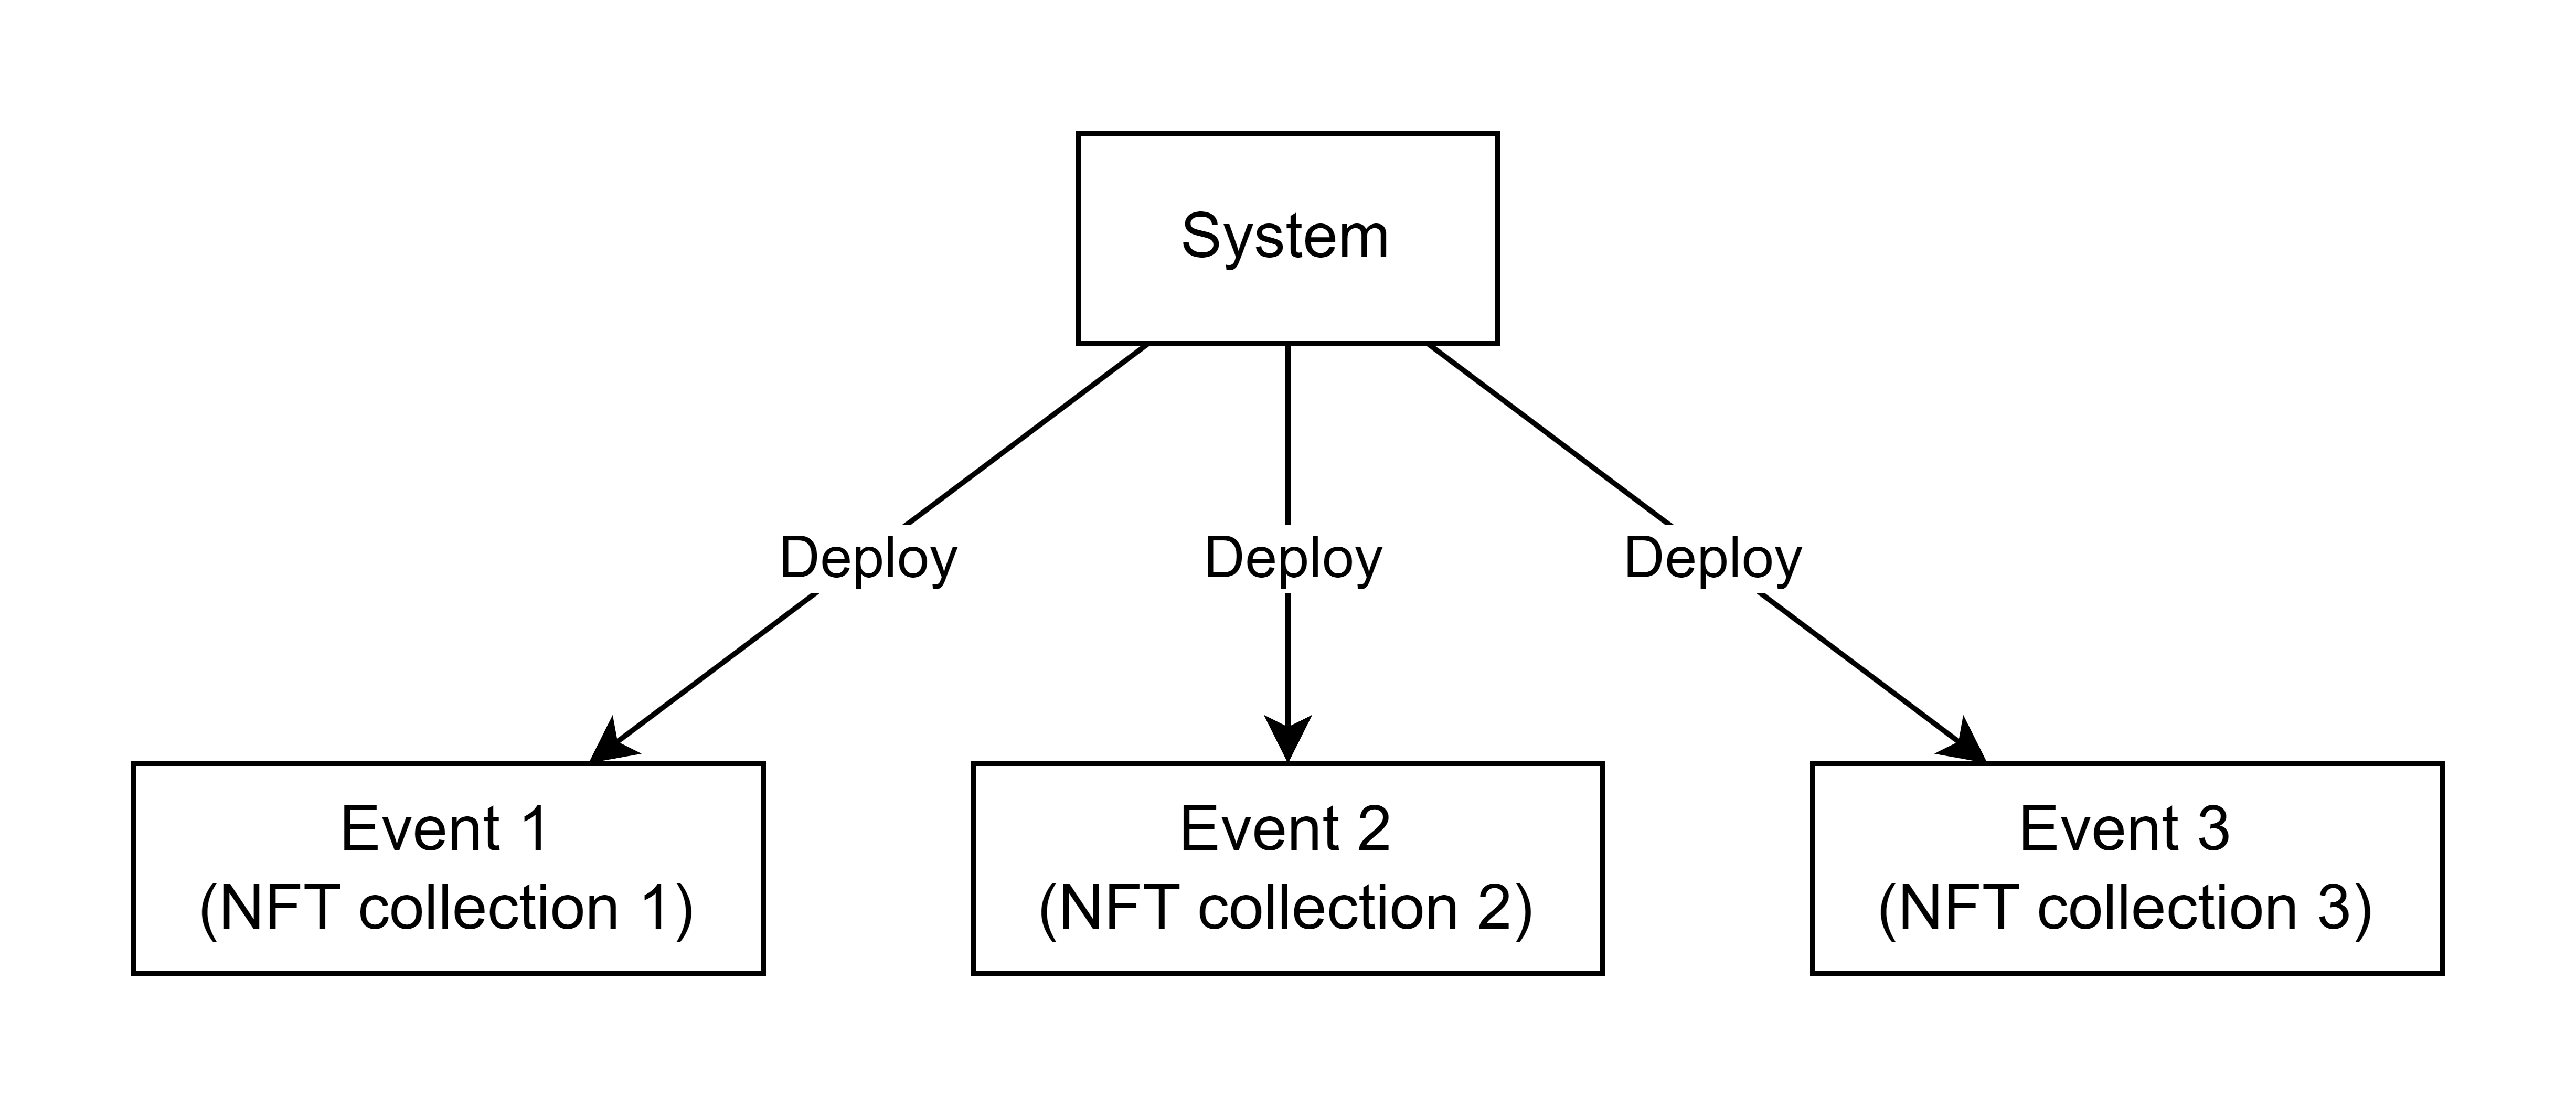
\includegraphics[width=\textwidth*2/3]{System behavior.png}
    \centering
    \caption{System behavior}
    \label{fig:system_behavior}
\end{figure}

With this in mind, like we see in the Figure \ref{fig:system_uml}, the main contract will track the organizers and the events associated with the system, along with the method to register a new event with the necessary data, restricted to only organizers (to avoid unauthorized people to interact).

\begin{figure}[H]
    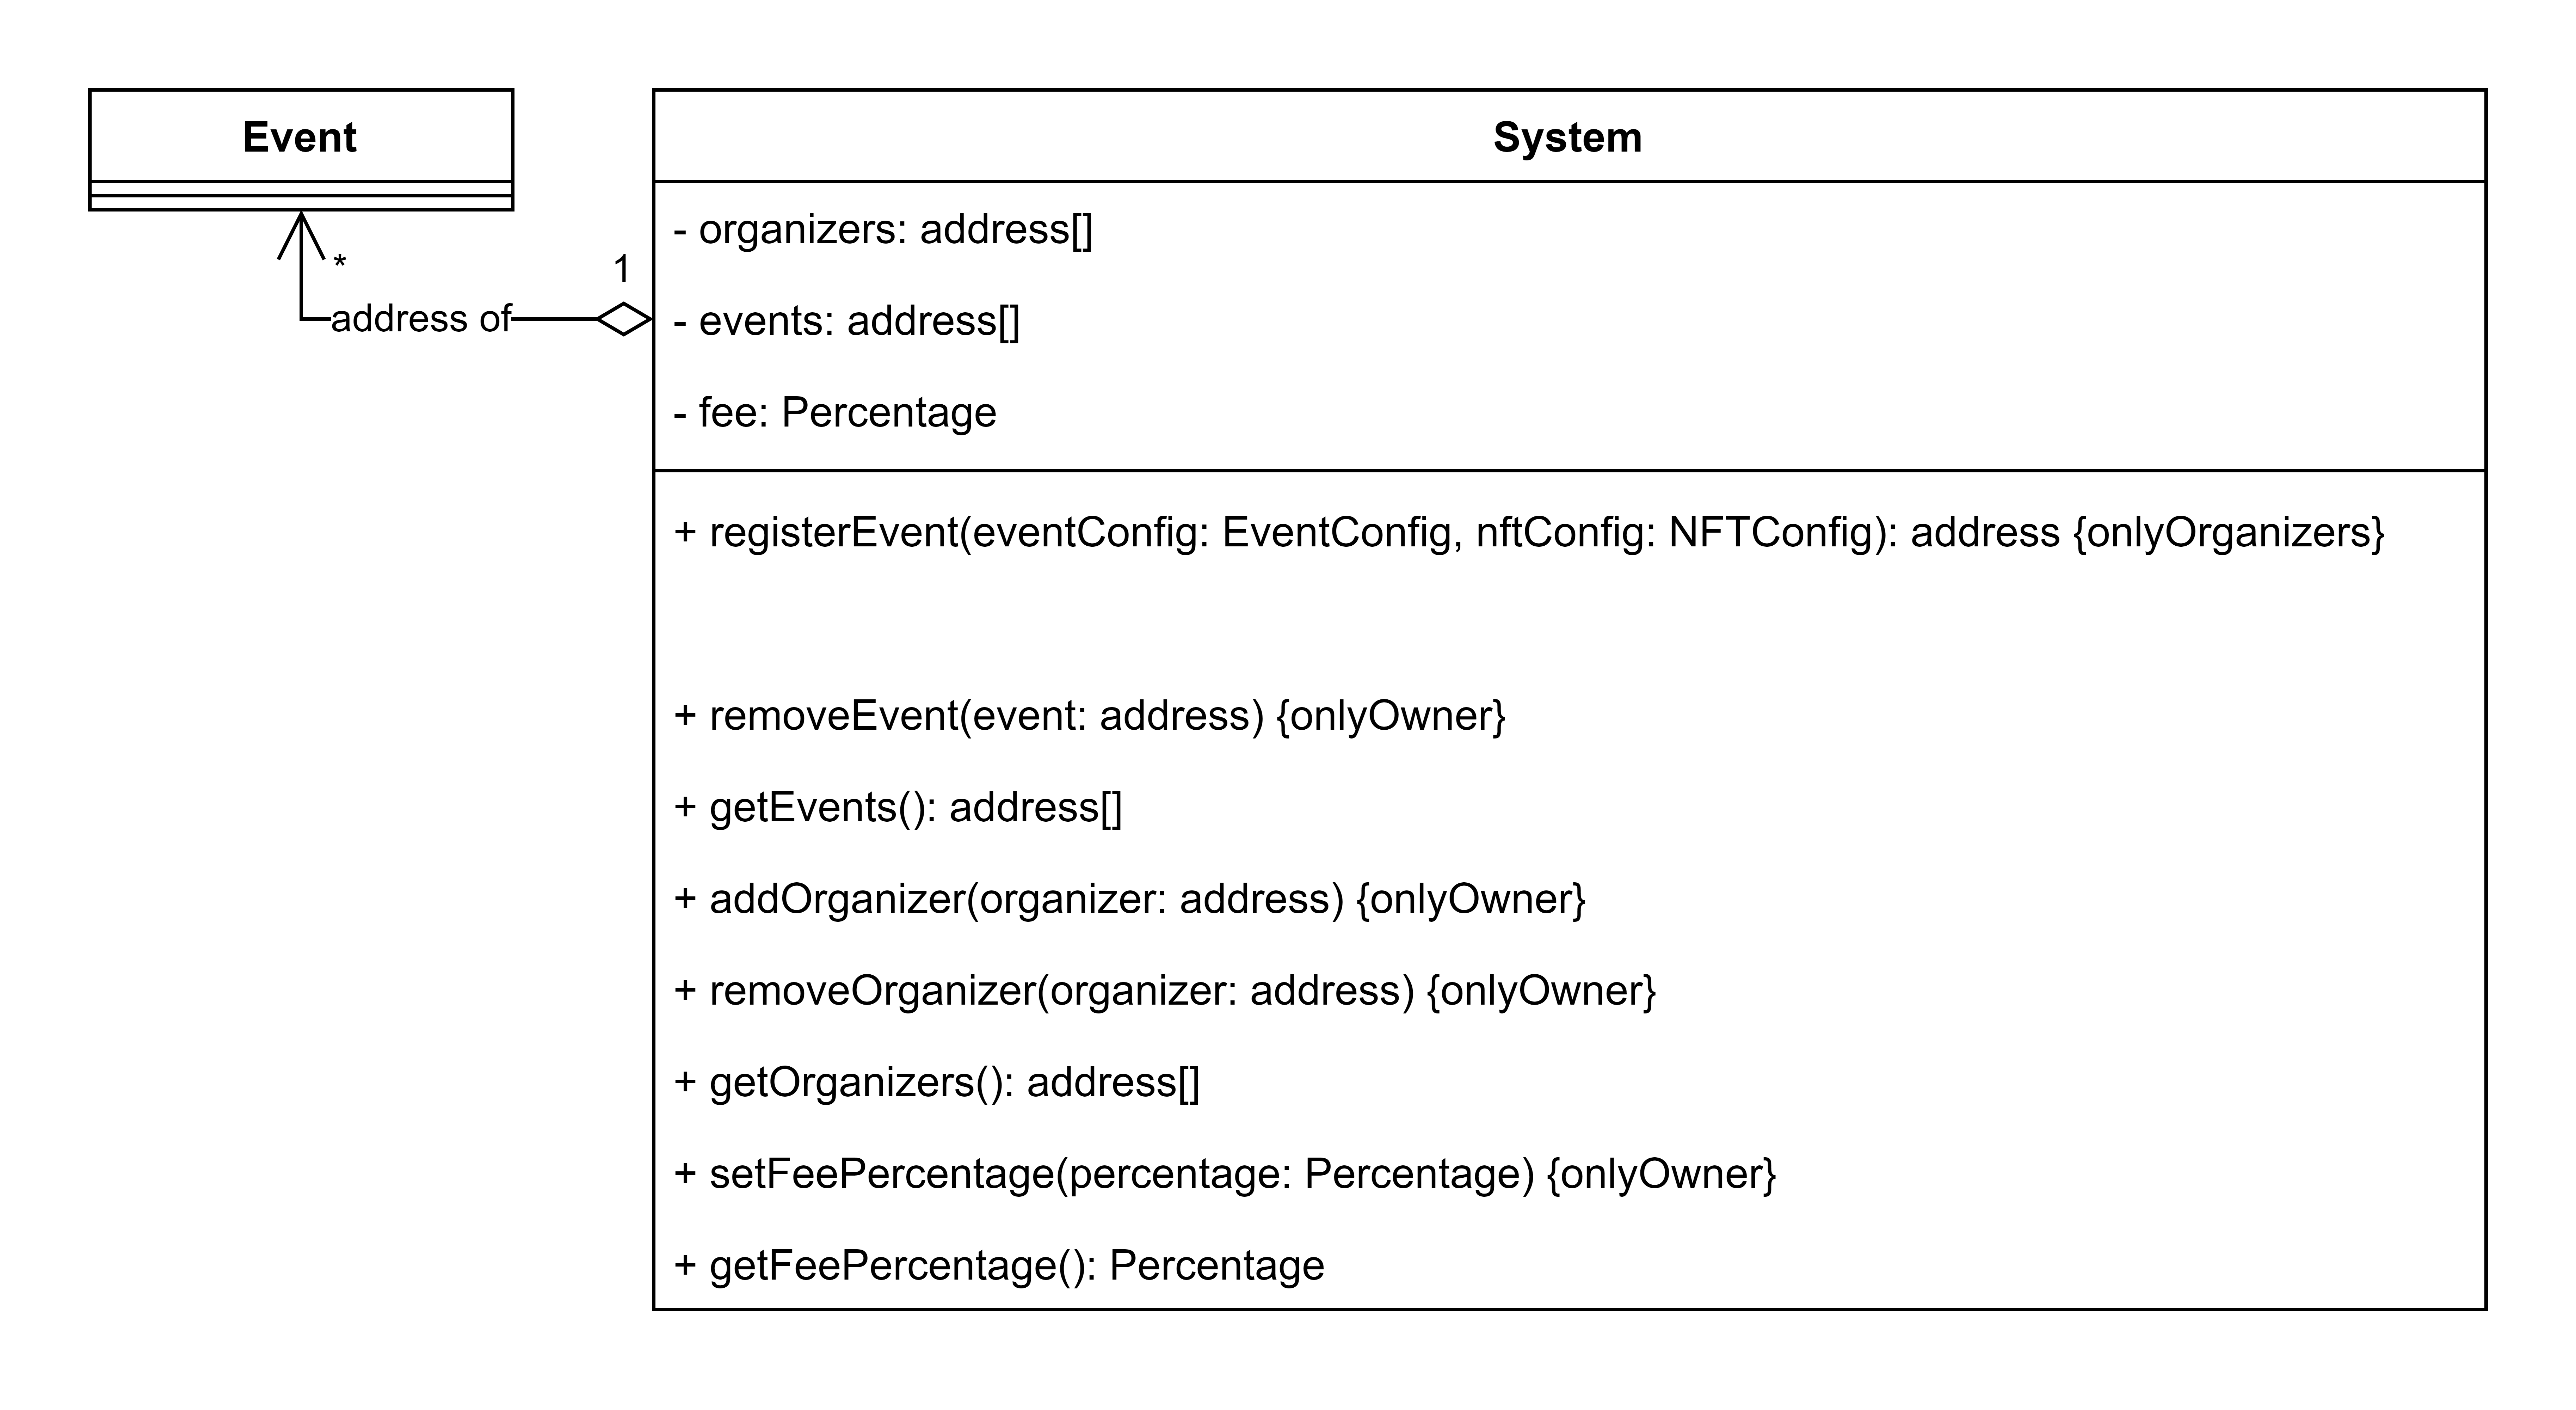
\includegraphics[width=\textwidth]{System UML.png}
    \centering
    \caption{Main smart contract UML}
    \label{fig:system_uml}
\end{figure}

With this structure, since we have this main contract where all the events of the system are stored, we can simply make a call to get them all, showcasing them in the app's home page for users to search. Any event that is deployed outside the system or if it gets removed from there, it won't be shown to the users.

\section{Event Smart Contract}
\label{sec:event_smart_contract}

For the event contract, we'll be extending the ERC721 standard and adding the necessary methods to interact with the tickets, like buying, selling, and validating them. The reason to extend this standard and not implement the logic manually is because it makes it compatible with the most common marketplaces for NFTs, which allows for users to do what they desire with them after the event. It also has the necessary methods to manage the tickets, like transferring them between users, and the necessary operations to track these operations.

\subsection{ERC721 Structure}
\label{subsec:erc721_structure}

The standard was obtained through the \href{https://docs.openzeppelin.com/contracts/api/token/erc721#ERC721}{OpenZeppelin} library, which is a collection of secure and community-vetted smart contracts that are used by many projects in the Ethereum ecosystem. This library is a great resource for developers to build secure and reliable smart contracts.

Analyzing its source code [ref], and looking into the most important variables and methods of the standard shown in the Figure \ref{fig:erc721_uml}, we can understand that the NFTs are simply a mapping of the token ID to the owner address, so when you execute a transaction to get a token (this process is called minting), the token ID is then associated to your address. Then for each token it's possible set a URI, which is a link to the NFTs metadata, usually being a JSON file with the necessary information about the token, like the name, description, and image.

This link could point to anything, for example a google drive file, but the common thing is to store the metadata on the IPFS, which is a decentralized storage system, so the metadata is not stored on the blockchain itself (onchain), which would be very expensive, but rather on a decentralized storage system (offchain), which is much cheaper.

\begin{figure}[H]
    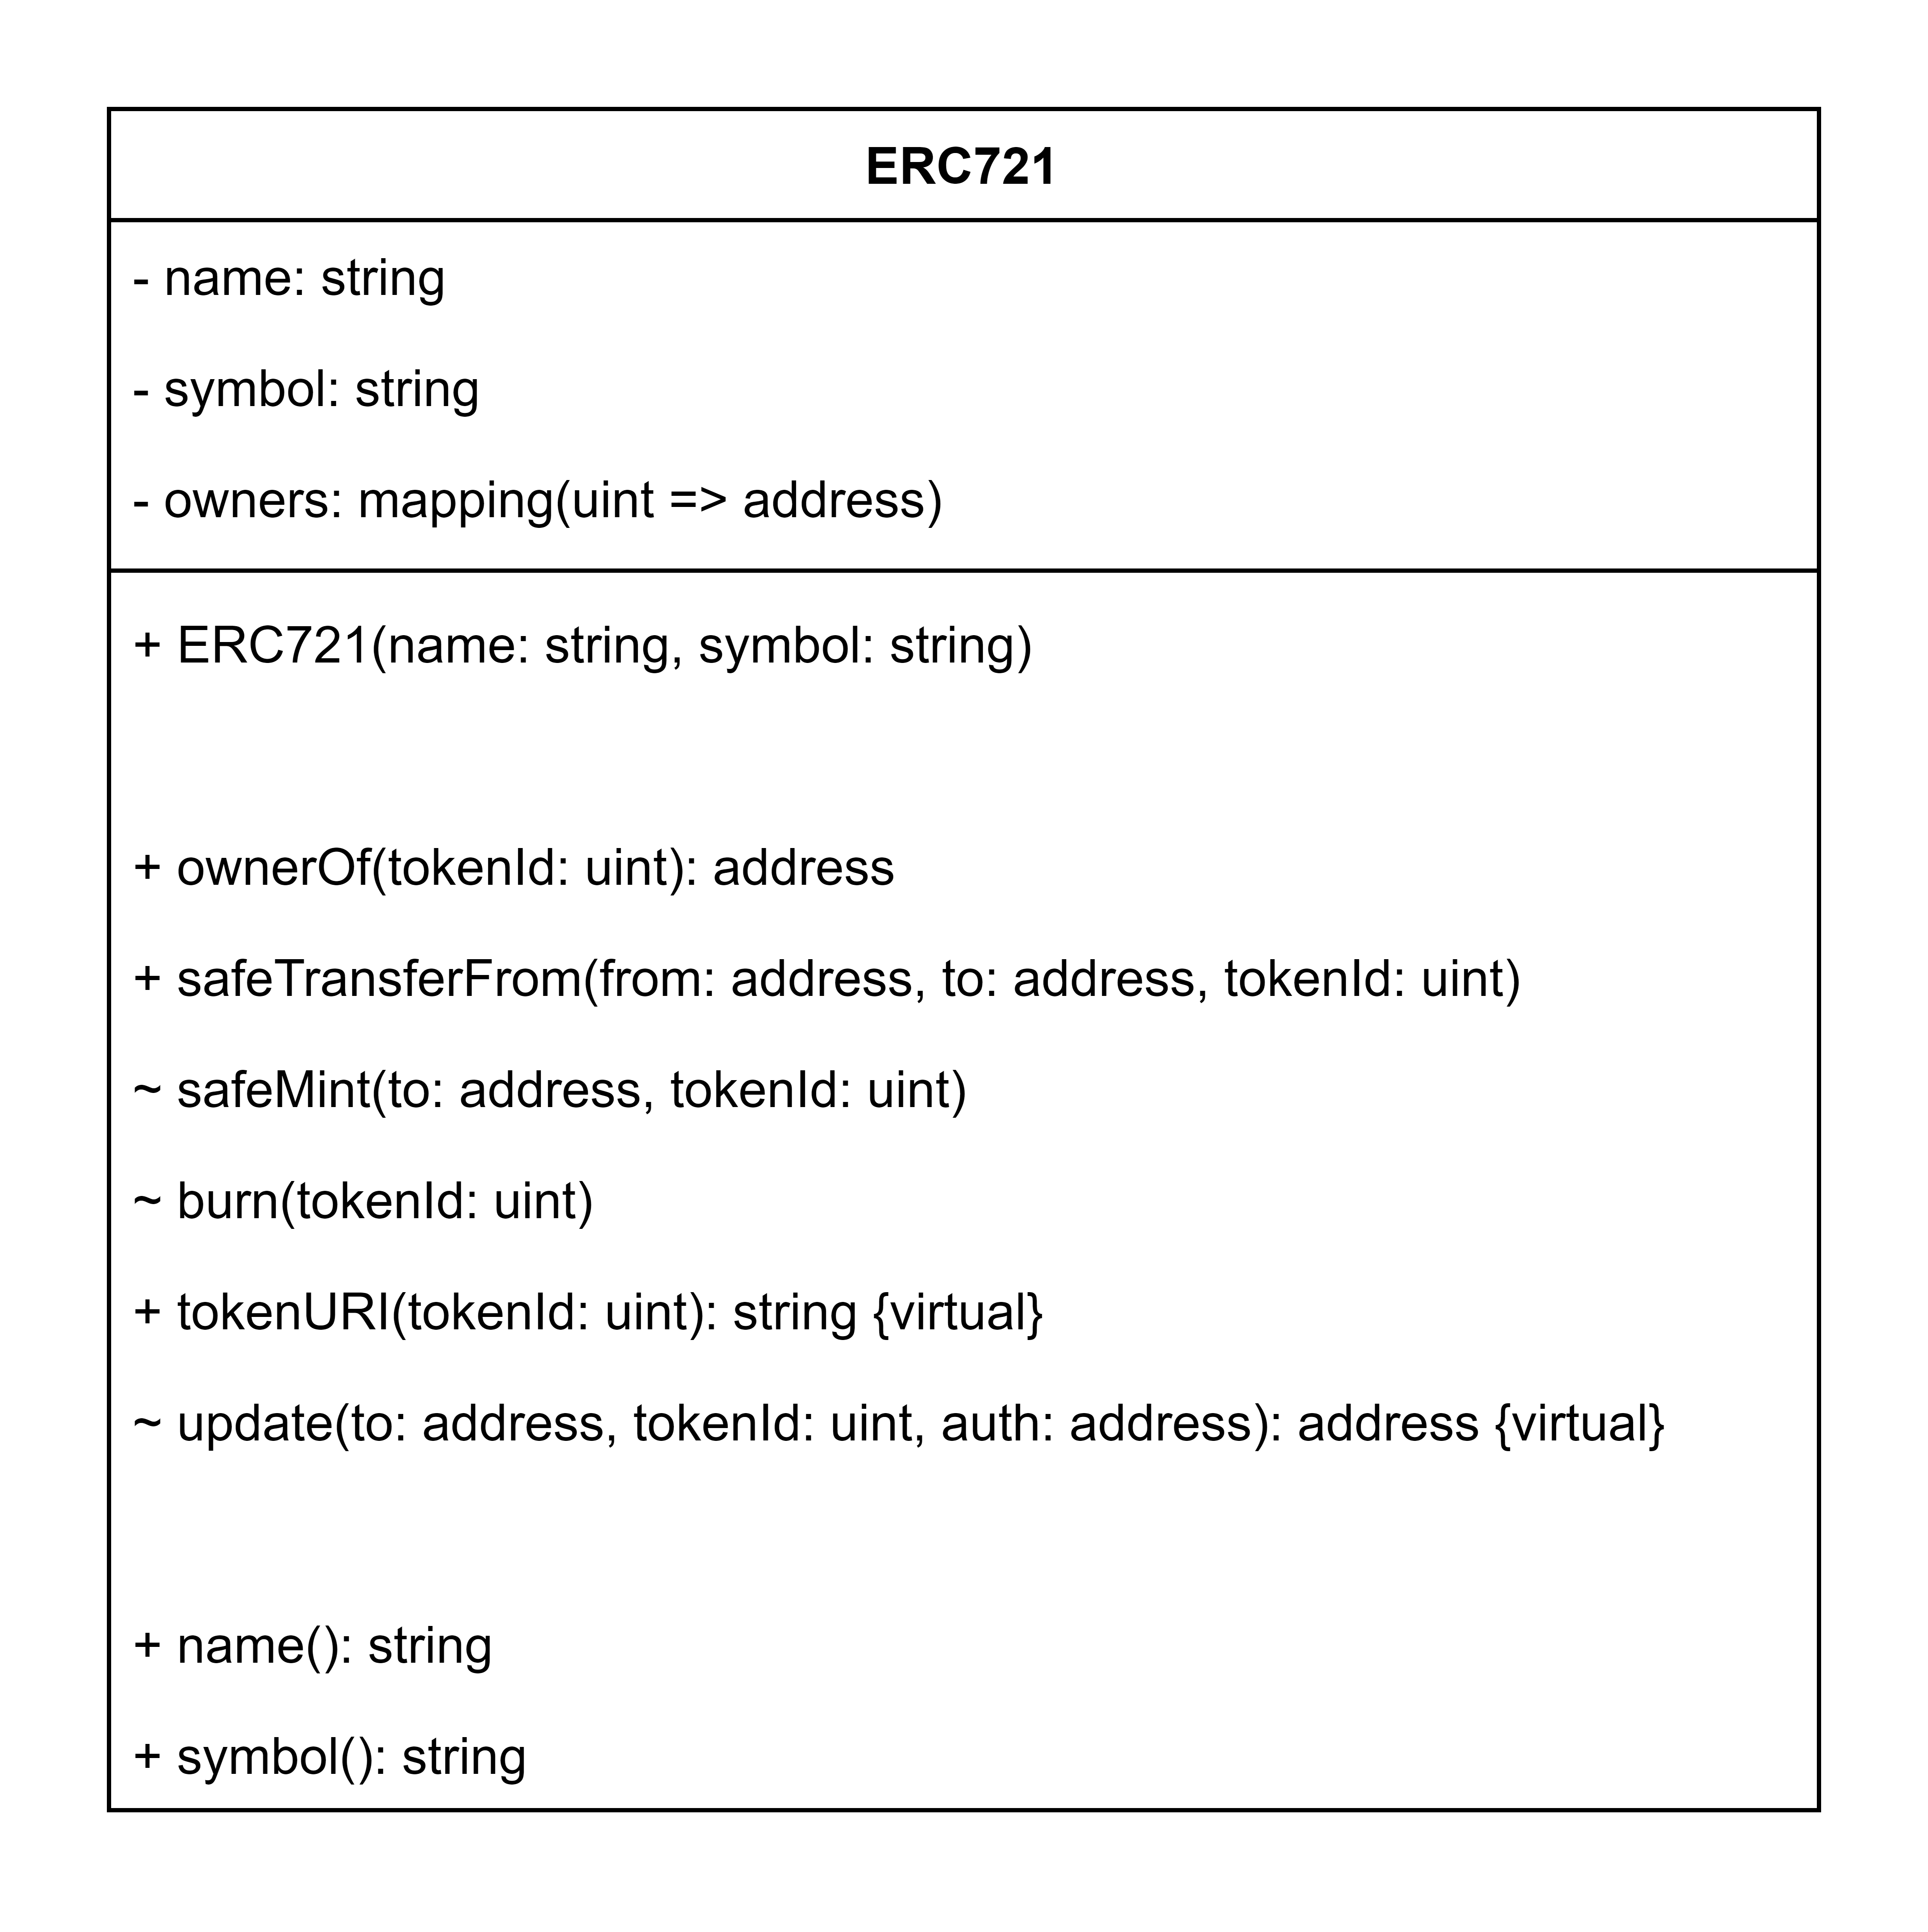
\includegraphics[width=\textwidth*2/3]{ERC721 UML.png}
    \centering
    \caption{ERC721 UML}
    \label{fig:erc721_uml}
\end{figure}

The function \textit{tokenURI} is the one that is called by default in the marketplaces to get the NFT's metadata, being one of the main reasons to extend the ERC721 standard, because it enforces the implementation of this method. In the Figure \ref{fig:erc721_uml} we see that it has the \textit{virtual} keyword, meaning this can be overridden by the contracts that extend it, to manipulate the way to store the metadata. We'll be mentioning this again in the Section \ref{fig:package_logic}, about how the packages logic is implemented.

\subsection{Event Behavior}
\label{subsec:event_behavior}

So the event will be deployed and we need a certain control over the tickets. One of the aspects we need to account for is that when deploying an event, and since the event will extend the ERC721, any public functions on that standard will be possible to execute. This is a problem because we don't want the users to mint tickets whenever they want or transfer them between themselves from outside the system, so we need to restrict these operations. As we saw already on the Figure \ref{fig:erc721_uml}, only the \textit{safeTransferFrom} method is public, so users could transfer NFTs between each other. We want that to be possible, just not from outside the system, since that can lead users to exploit the system and scalping the tickets easily. The minting, however, won't be an issue because it's an internal method, so we will access it from the buy method in the event and restrict it there.

The Figure \ref{fig:event_lifecycle} shows the lifecycle of the event, and what restrictions are in place for the ticket operations. We will have 4 main states for the event after it has been registered, being \textit{Open}, \textit{No refund}, \textit{Start}, and \textit{End} dates. Once the event is registered, it will show up in the app for user to see, and the organizers can set a later open date to allow ticket minting (buying).

\begin{figure}[H]
    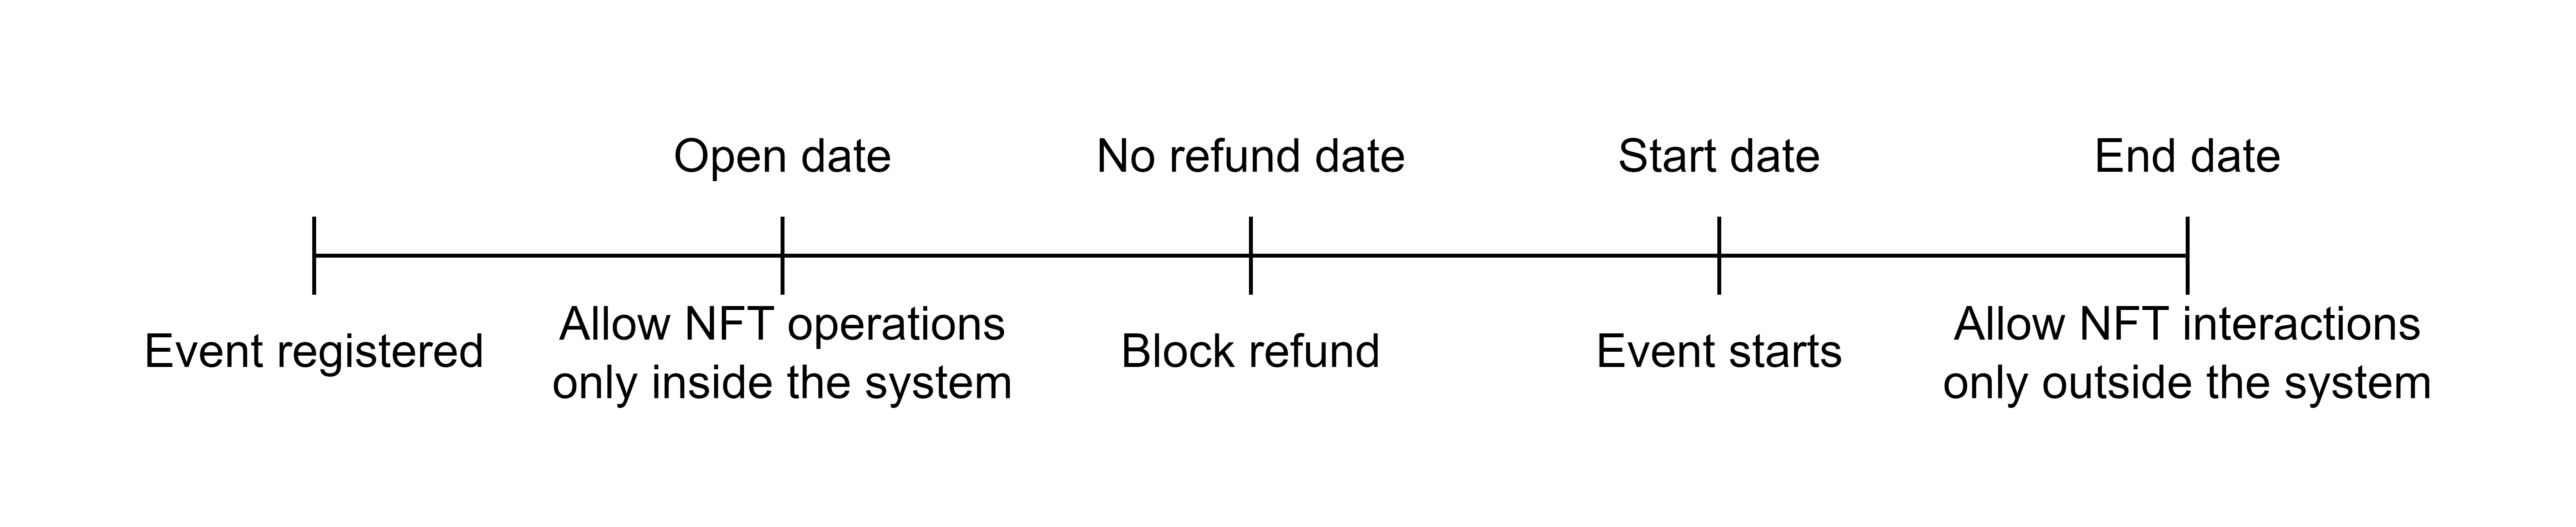
\includegraphics[width=\textwidth]{Event lifecycle.png}
    \centering
    \caption{Event lifecycle}
    \label{fig:event_lifecycle}
\end{figure}

\subsubsection{Open Date}

Once it hits the \textit{Open} date, we will allow the users to buy the tickets, which will mint the NFTs by executing the \textit{safeMint} method of the ERC721 contract.

\subsubsection{No Refund Date}

After the \textit{No refund} date, we will prevent the users to call the refund method, which essentially \textit{burns} the NFTs, removing them from the user and making them available again.
This is a nice operation to add because it allows the users to get their money back if they can't attend the event. The organizer decides the percentage of the refund and the deadline, which is there to prevent users to buy a big amount of tickets and then refund them last minute, which would be a way to exploit the system (in case of a 100\% refund, they wouldn't risk anything).
The other good thing for the organizer is when the event is expected to be sold out. Since the users will get some money back, they will have a reason to refund their tickets if they cannot attend the event anymore, making them available again for other users to buy at the original price, making the organizer a higher profit.
After this deadline, the only that'll be allowed is for users to resell their tickets in the system's marketplace, which them to sell at a higher price than the refund (but never higher than the original, of course).

\subsubsection{Start Date}

The \textit{Start} date is there to tell the users when the event starts, so basically when the gates will open. That's the date that appears in the app, so the users know when to show up.

\subsubsection{End Date}

The \textit{End} date tells when the event is over, unlocking all the ticket operations to outside the system. So users can simply keep the tickets as a souvenir or sell them in any marketplace, without any restrictions on the tickets, including the elimination of the price cap.

With this behavior in mind, we came up with the Event UML, like shown in the Figure \ref{fig:event_uml}, where we added the necessary methods for the organizer/admins to manage the event and the users to handle the tickets, which then trigger the corresponding methods of the ERC721 contract. We added a possibility to have admins so the organizer can distribute the workload of executing the necessary operations to people he trusts.

\begin{figure}[H]
    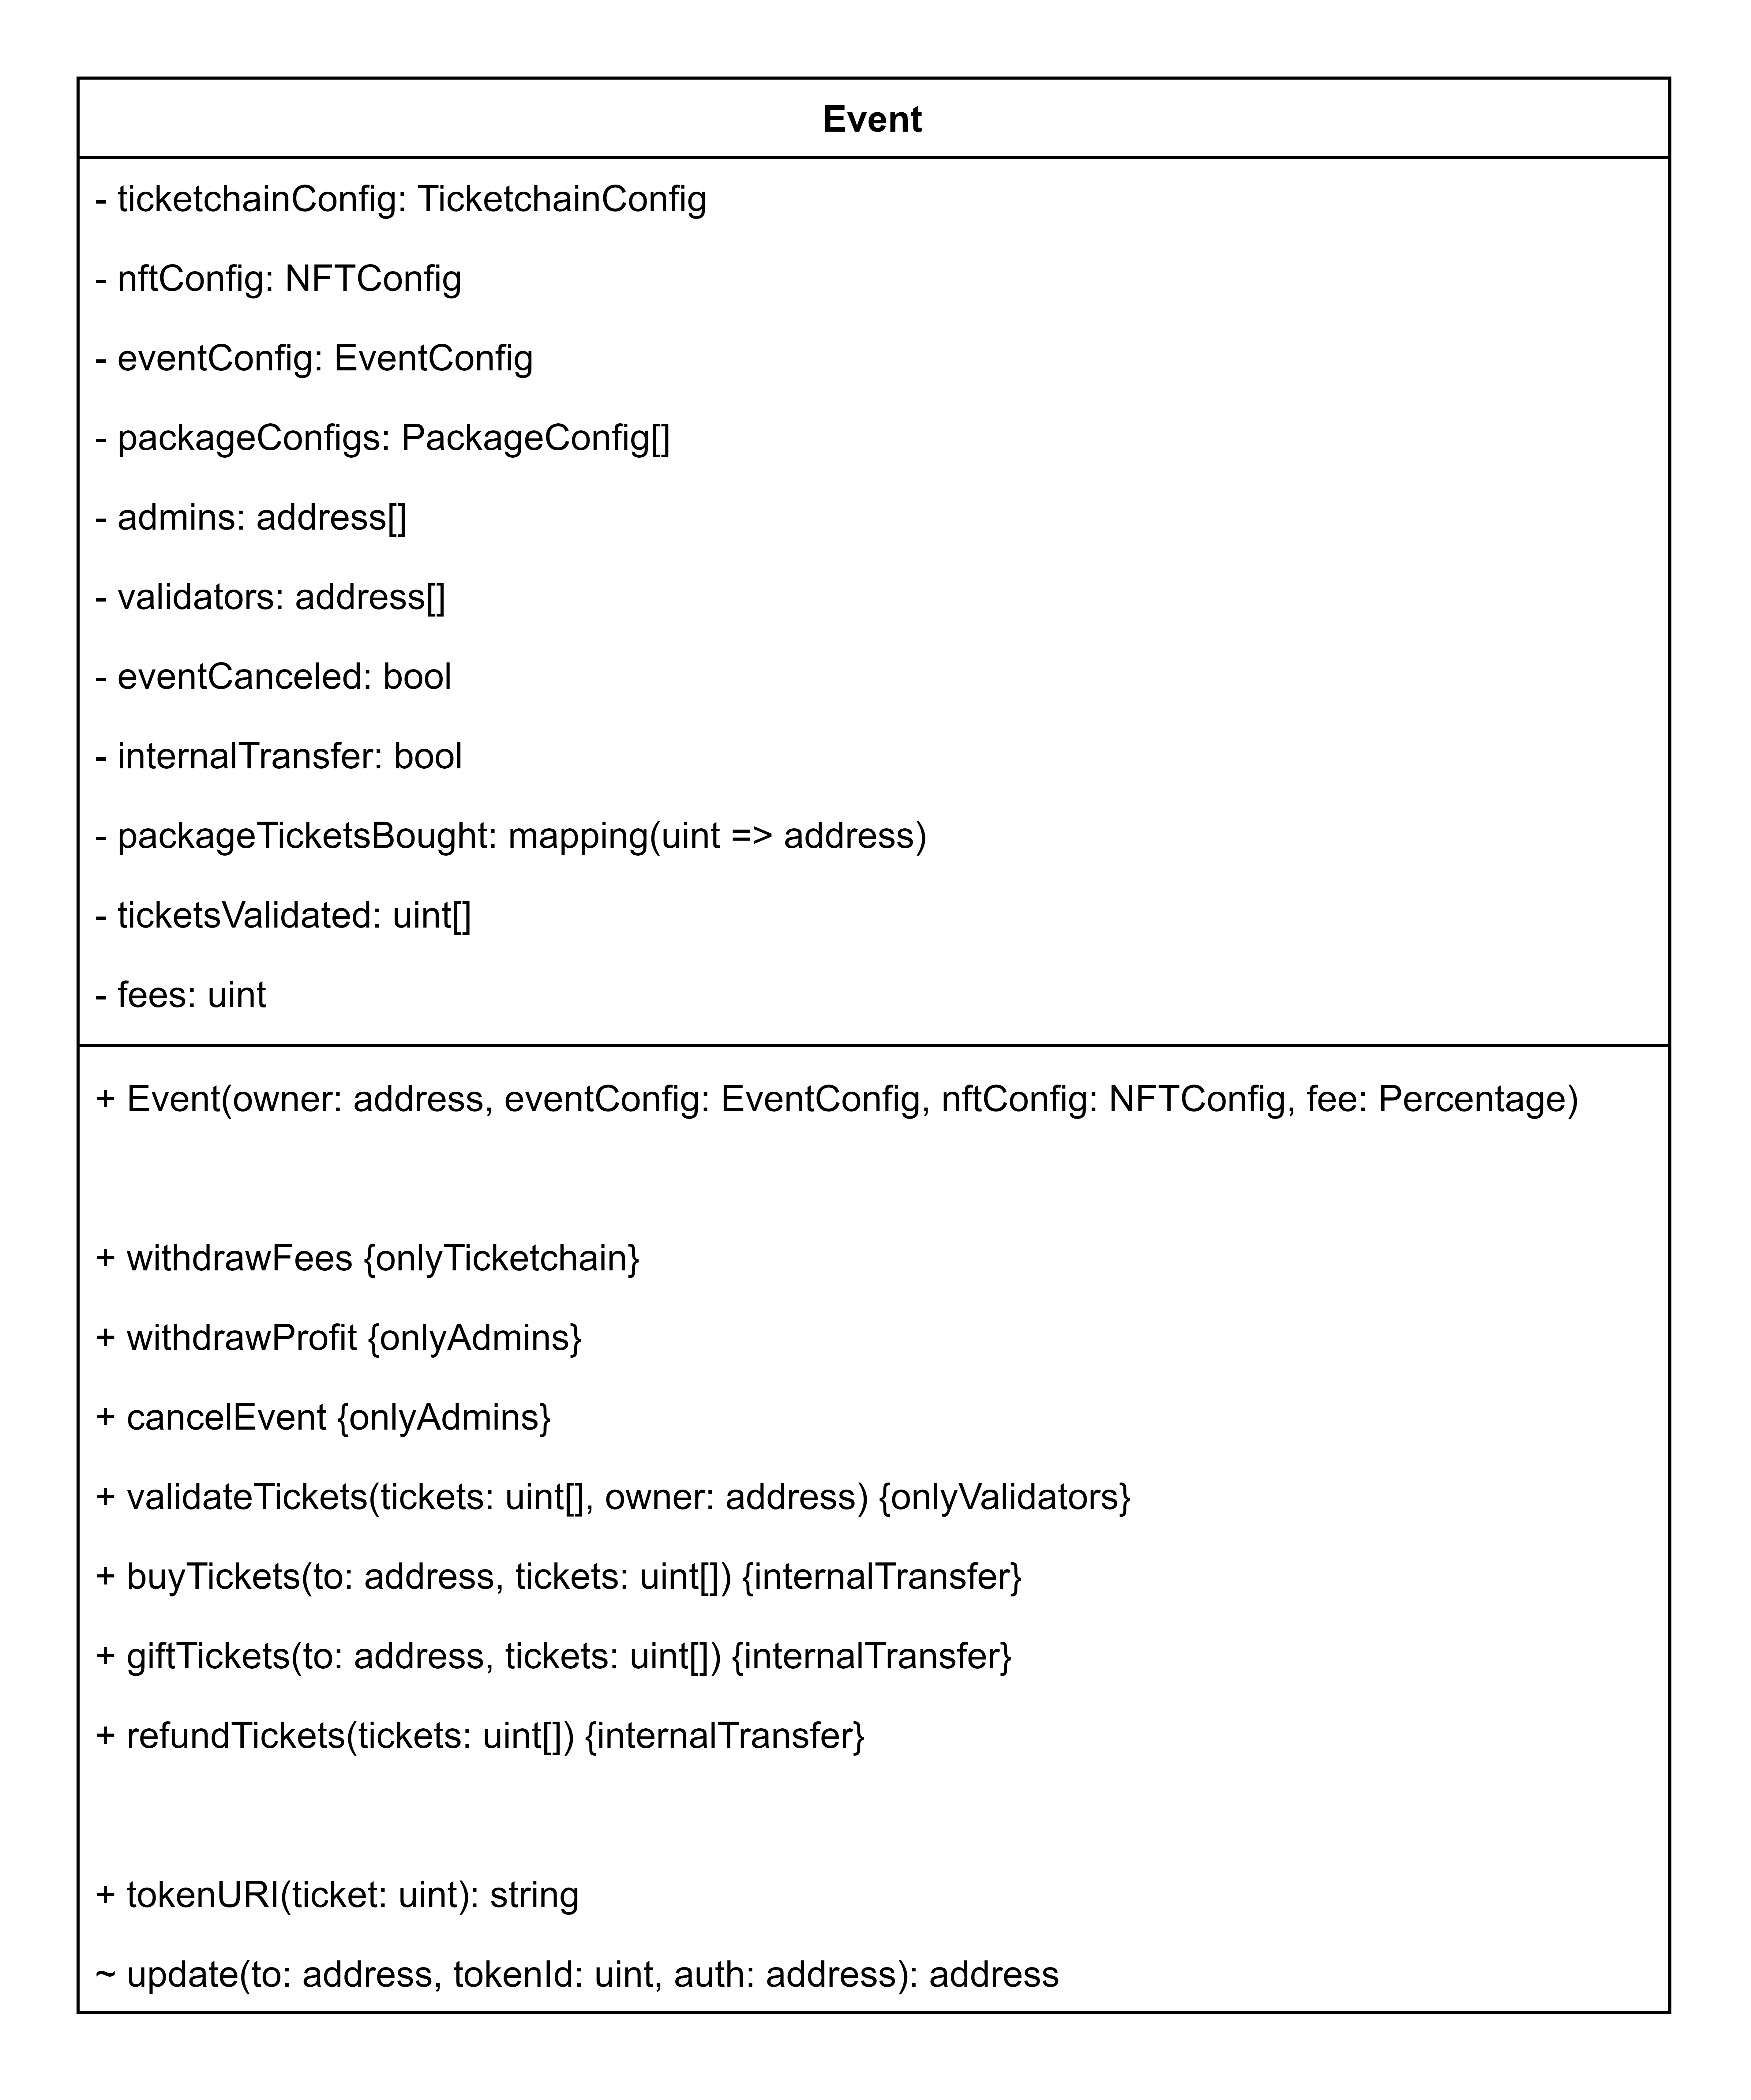
\includegraphics[width=\textwidth*3/4]{Event UML.png}
    \centering
    \caption{Event smart contract UML}
    \label{fig:event_uml}
\end{figure}

\subsection{Structs}
\label{subsec:structs}

As is possible to see in the Figure \ref{fig:event_uml}, and also in the Figure \ref{fig:system_uml}, we have a few custom structs to organize better the data. These structs are the \textit{Percentage}, \textit{EventConfig}, \textit{NFTConfig}, \textit{PackageConfig} and \textit{TicketchainConfig} structs.

\subsubsection{Percentage Struct}

The \textit{Percentage} struct is necessary because in Solidity there are no floating point numbers, so we need a way to make calculations with percentages. What this struct does is it stores the value of the percentage and the amount of decimals it has, so if we want to calculate 55.50\% of a number, we would have 555 as the value with 1 decimal, or 5550 with 2 decimals.

The struct is as follows:
\begin{verbatim}
    struct Percentage {
        uint256 value;
        uint256 decimals;
    }
\end{verbatim}
so to obtain a percentage of some $x$ number, we do $y = \frac{x \times \text{Percentage.value}}{100\mathrm{e}^\text{Percentage.decimals}}$.

When working with ether units, it can be common to have values like 0.00005 ether, but it's rather rare to have small values in wei, like 1000 wei, so applying this formula won't lose much precision (note that 1 ether is $10^{18}$ wei).

\subsubsection{TicketchainConfig Struct}

The \textit{TicketchainConfig} struct is simply to keep it stored the system address and the system fee percentage, so we can easily access this information when applying the fees and withdrawing them, and is as follows:
\begin{verbatim}
    struct TicketchainConfig {
        address ticketchainAddress;
        Percentage feePercentage;
    }
\end{verbatim}

\subsubsection{NFTConfig Struct}

The \textit{NFTConfig} struct is just to store the NFTs basic information, like the name, symbol, and base URI, to ease the input of the NFTs information when registering the event:
\begin{verbatim}
    struct NFTConfig {
        string name;
        string symbol;
        string baseURI;
    }
\end{verbatim}

\subsubsection{EventConfig Struct}

The \textit{EventConfig} struct is to store the event's entire configuration, like the name, description, location, dates, and refund, like this:
\begin{verbatim}
    struct EventConfig {
        string name;
        string description;
        string location;
        uint256 openDate;
        uint256 noRefundDate;
        uint256 startDate;
        uint256 endDate;
        Percentage refundPercentage;
    }
\end{verbatim}

\subsubsection{PackageConfig Struct}

Lastly, the \textit{PackageConfig} struct is there to store each package information, to keep track of the ones that are available for the event:
\begin{verbatim}
    struct PackageConfig {
        string name;
        string description;
        uint256 price;
        uint256 supply;
        bool individualNfts;
    }
\end{verbatim}
This structure will be better discussed in the next Section \ref{subsec:ticket_packages}.

\subsection{Ticket Packages}
\label{subsec:ticket_packages}

It's common to see events with different types of tickets, like VIP, standard, or even 3-day passes, each with its own price and benefits. We want to implement this feature in the system, so we can have a better control over the tickets and the users can choose the one that fits them better.

For that, we will allow the organizer to add packages, indicating the supply of each one, and as we saw already, the NFTs are a mapping of the ID to the owner, so we can organize the packages as a list, where the supply and order of the package defines the ID of each NFT, like the Figure \ref{fig:package_logic} demonstrates.

\begin{figure}[H]
    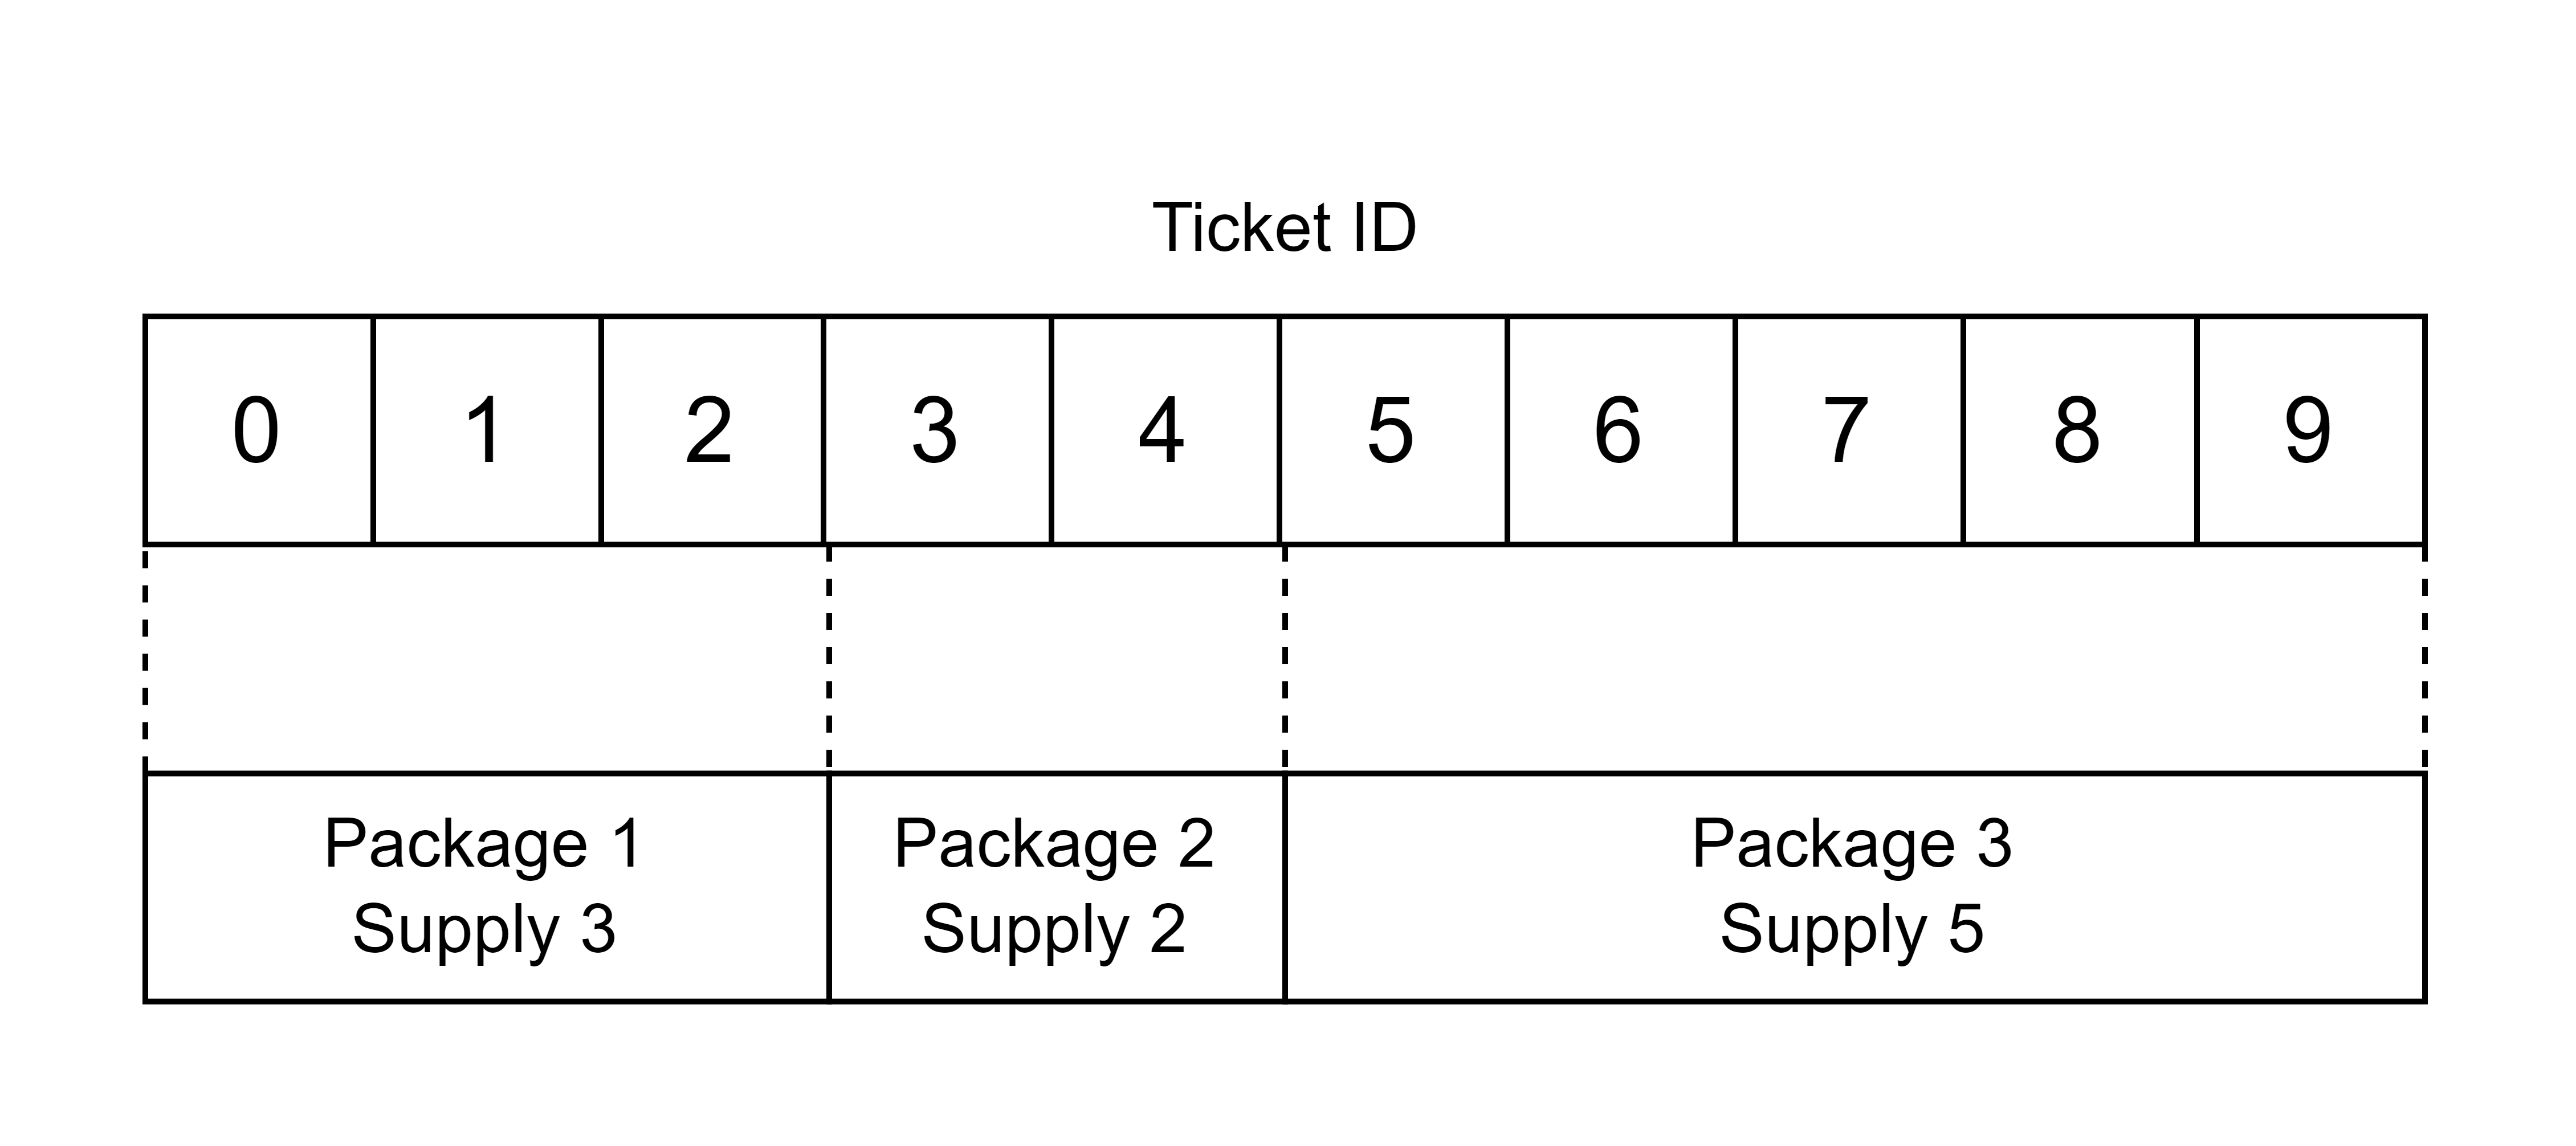
\includegraphics[width=\textwidth*2/3]{Package logic.png}
    \centering
    \caption{Package logic}
    \label{fig:package_logic}
\end{figure}

This way, whenever we need to get a ticket for a certain package, we can go through the packages and see in which one the ID is. One only limitation with this is if the event is already open (users can buy tickets), the only thing we can allow the organizer to do is to add packages, neither remove or change their order, because that would change the ID of the ticket, which would be a problem for the users that already bought them.

    [mention how tokenURI was implemented]

\subsection{System Fees}
\label{subsec:system_fees}

One of the most important aspects of a system like this is the business model we have to take into account. Since this is a service we want to deploy for event organizers, we need to make this sustainable and profitable. This kind of service aims to do some heavy lifting, with its own features, so we could set a fee lower than the usual on the traditional marketplaces and ticket selling platforms, since the organizers need to pay for each service.

These low fees are possible because with the system being deployed on the blockchain, it stays there while the network is running, so the only extra cost are the network fees when interacting with the event. For the users, each interaction is paid by them, so when a user buys a ticket, the only thing to take into account are the network fees, which depending on the network can be super low.

We'll set a fee on the main smart contract, where will be stored in the event when registering it, so that if we decide to change it, the previous events aren't affected. This is also because we want to abstract the user of any extra fee, so the price the organizer sets, is the price the user pays, and the system fee is taken from the tickets price. In case an event gets cancelled, or a user decides to get a refund, the ticket fee is returned to the user (proportional to the refund), making the system less profit, but guarantees the users of a fair process. With this, we need to restrict the system to only withdraw any profit when the event is over. Since this is rather an uncommon case, the less profit for the system is worth the trust the users and organizers will have in it.

~

[NOTES]

~

[mention storage]
-- [ipfs (pinata)]

- [restrictions on ticket operations]

[ticket validation]
[todo mention network fees and network choice]

[user app]
[validator app]

\section{Project Features}
\label{sec:project_features}
